\RequirePackage{fix-cm}
\documentclass[11pt]{article}
\usepackage[margin=1in]{geometry}
\usepackage{fancyhdr}
\usepackage{enumitem}
\usepackage{parskip}
\usepackage{graphicx}
\usepackage{needspace}

\pagestyle{fancy}
\fancyhf{}
\fancyhead[C]{\textbf{SEG2105}}
\fancyfoot[C]{\thepage}
\setlength{\headheight}{14pt}
\setlength{\emergencystretch}{2em}

\newcounter{chapterNumber}
\setcounter{chapterNumber}{3}
\newcounter{headerOneCount}
\newcounter{headerTwoCount}[headerOneCount]
\setcounter{headerOneCount}{-1}
\renewcommand{\theheaderOneCount}{\arabic{headerOneCount}}
\renewcommand{\theheaderTwoCount}{\arabic{headerTwoCount}}

\newcommand{\Title}[1]{%
  \begin{center}
    \fontsize{16}{28}\selectfont\textbf{#1}
  \end{center}
}

\newcommand{\HeaderOne}[1]{%
  \Needspace{5\baselineskip}
  \refstepcounter{headerOneCount}%
  \setcounter{headerTwoCount}{-1}%
  {\noindent\fontsize{14}{22}\selectfont\textbf{\arabic{chapterNumber}.\theheaderOneCount\ #1}\par}
}

\newcommand{\HeaderTwo}[1]{%
  \Needspace{5\baselineskip}
  \refstepcounter{headerTwoCount}%
  {\noindent\fontsize{14}{20}\selectfont\textbf{\arabic{chapterNumber}.\theheaderOneCount.\theheaderTwoCount\ #1}\par}
}

\newcommand{\BodyText}[1]{%
  \fontsize{11}{15}\selectfont #1\par

}

\newenvironment{NumberedList}{%
  \begin{enumerate}[leftmargin=2em, itemsep=0.35em, topsep=0.35em]
}{%
  \end{enumerate}
}

\newenvironment{DottedList}{%
  \begin{itemize}[leftmargin=2em, itemsep=0.35em, topsep=0.35em, label=\textbullet]
}{%
  \end{itemize}
}

\begin{document}
\Title{Chapter 3: Basing Software Development on Reusable Technology}

\HeaderOne{Building on the Experience of Others}
\BodyText{Why Build X When Y Exists?}
Types of reuse:
\begin{DottedList}
  \item Expertise
  \item Standard designs and algorithms
  \item Libraries of classes or procedures
  \item Powerful commands built into languages and operating systems
  \item Frameworks
  \item Complete applications
\end{DottedList}

\HeaderOne{Frameworks: Reusable Subsystems}
\BodyText{A framework is reusable software that implements a generic solution to a generalized problem}
\textbf{Principle: Applications that do different (but related) things tend to have similar designs}

\HeaderTwo{Frameworks to promote reuse}
\BodyText{\textbf{A framework is inherently \textit{incomplete}}}
\begin{DottedList}
  \item Certain classes or methods are used by the framework but are missing (slots)
  \item Some functionality is optional, requiring implementation by the dev
  \item Developers use services provided by the framework. \textbf{Services are called the API}
\end{DottedList}

\HeaderTwo{Object-oriented frameworks}
\BodyText{\textbf{In the object oriented paradigm, a framework is composed of a library of classes.}}
\begin{DottedList}
  \item The API is defined by the set of all public methods of these classes
  \item Some of the classes will normally be abstract and there are often many Interfaces
\end{DottedList}

\newpage
\HeaderTwo{Frameworks and product lines}
\BodyText{A product line (or product family) is a set of products built on a common base of technology}
\begin{DottedList}
  \item The various products in the product line have different features to satisfy different markets
  \item The software common to all products is included in a framework
  \item Each product is produced by filling the available hooks and slots
\end{DottedList}
\HeaderTwo{Types of frameworks}

\begin{DottedList}
  \item A \textit{horizontal} framework provides general application facilities that a large number of applications can use
  \item A \textit{vertical} framework (application framework) is more 'complete' but still needs some slots to be filled to adapt it to specific application needs
\end{DottedList}
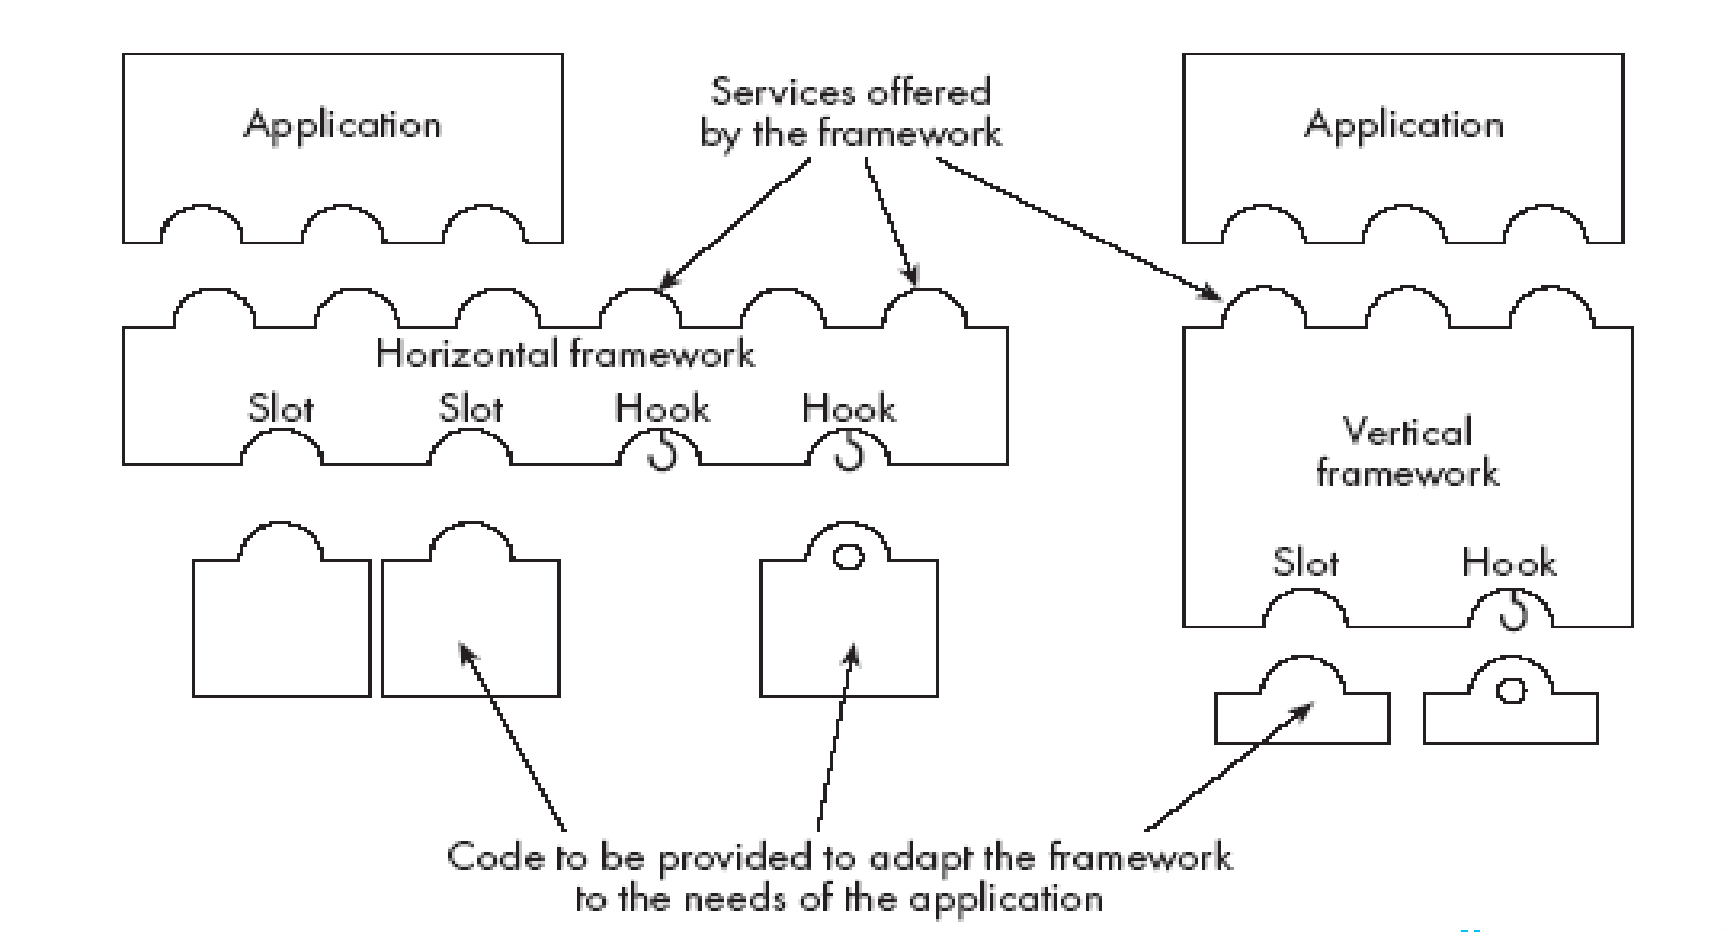
\includegraphics[width=1\textwidth]{Figure1.png}
\begin{center}
  \BodyText{Figure 1: Horizontal vs Vertical Framework}
\end{center}

\newpage
\HeaderOne{The Client-Server Architecture}
\BodyText{\textbf{A \textit{Distributed system} is a system in which:}}
\begin{DottedList}
  \item Computations are performed by separate programs
  \item processes normally run on separate machines
  \item machines and programs cooperate to perform the task of the system
\end{DottedList}
\BodyText{\textbf{Server:}}
\begin{DottedList}
  \item A program that provides a service for other programs that connect to it using a communication channel
\end{DottedList}
\BodyText{\textbf{Client:}}
\begin{DottedList}
  \item A program that accesses a server (or multiple) to obtain services
  \item Multiple clients may access a server simultaneously
\end{DottedList}
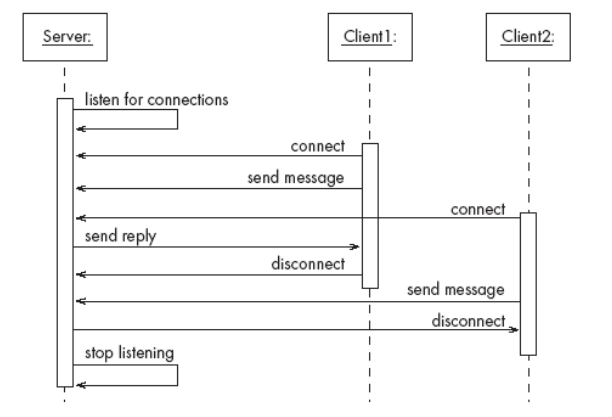
\includegraphics[width=1\textwidth]{Figure2.png}
\begin{center}
  \BodyText{Figure 2: A server program communicating with two client programs}
\end{center}

\newpage
\HeaderTwo{Activities of a server}

\begin{NumberedList}
  \item Initializes itself
  \item Starts listening for clients
  \item Handles the following types of events originating from clients
  \begin{NumberedList}
    \item accepts connections
    \item responds to messages
    \item handles client disconnections
  \end{NumberedList}
  \item May stop listening
  \item Must cleanly terminate 
\end{NumberedList}

\HeaderTwo{Activities of a client}
\begin{DottedList}
  \item Initialize the client and initiate a connection.
  \item Send messages and handle replies, server disconnection, and communication failures.
  \item Close resources and terminate cleanly.
\end{DottedList}
\HeaderTwo{Threads, work distribution, and protocols}
\begin{DottedList}
  \item A server must accept connections while serving existing clients. OCSF separates the listening thread from client-connection threads.
  \item Thin clients delegate most processing to the server. Fat clients do more locally, potentially reducing server load.
  \item A protocol defines valid messages in each direction and rules for their exchange. Both sides must agree on content, order, and error handling.
  \item Design the application work, its distribution, messages, initialization, connection handling, and termination.
  \item Benefits include remote access, shared services, independent client/server development, and choices about central or distributed data.
\end{DottedList}
\HeaderOne{Technology Needed for Client-Server Systems}
\begin{DottedList}
  \item IP routes packets among hosts. TCP provides a reliable, ordered byte stream over a connection; it does not define application message boundaries.
  \item DNS resolves host names to addresses. localhost refers to the local machine, so a remote client needs the actual server address or host name.
  \item IPv4 addresses have 32 bits; IPv6 addresses have 128 bits.
  \item Clients need a server host and port. Port numbers range from 0 to 65535.
  \item System/well-known ports are 0-1023, registered/user ports are 1024-49151, and dynamic/private ports are 49152-65535. Actual ephemeral allocation depends on operating-system configuration.
  \item UDP sends datagrams without TCP's connection, reliable delivery, or ordering guarantees. It still has protocol overhead.
\end{DottedList}
\HeaderTwo{Connections and streams in Java}
\begin{DottedList}
  \item java.net.ServerSocket listens for connections. new ServerSocket(port) binds a listening socket; accept() waits and returns a separate Socket for the connected client.
  \item new Socket(host, port) attempts a TCP connection. It does not continually ping until accepted; connection attempts can fail with an exception.
  \item getInputStream() receives bytes and getOutputStream() sends bytes. Stream classes belong to java.io.
  \item DataInputStream and DataOutputStream encode primitive values. Pair matching methods in the same order, such as writeUTF with readUTF.
  \item ObjectInputStream and ObjectOutputStream exchange serialized objects. Peers must agree on compatible message types.
  \item Close connections and streams when finished, and handle failures rather than assuming the peer remains connected.
\end{DottedList}
\HeaderTwo{Local example}
\begin{DottedList}
  \item Client.java connects to localhost on port 8888, writes a UTF message, reads a UTF reply, and closes the socket.
  \item Server.java listens on port 8888, accepts one connection, reads a UTF message, writes a reply, and closes that connection.
  \item Serving multiple clients requires an accept loop and a strategy for handling each connection. Extending Thread alone does not start a background thread.
\end{DottedList}
\HeaderOne{The Object Client-Server Framework (OCSF)}
\begin{DottedList}
  \item OCSF supplies connection and communication behaviour through AbstractClient, AbstractServer, and ConnectionToClient.
  \item Extend intended abstract classes instead of modifying framework code.
  \item Services are methods application code calls. Slots are required methods subclasses implement. Hooks are optional callback methods subclasses may override.
\end{DottedList}
\HeaderOne{The Client Side}
\begin{DottedList}
  \item Subclass AbstractClient and implement handleMessageFromServer(Object msg).
  \item openConnection(), closeConnection(), and sendToServer(msg) control communication.
  \item isConnected(), getHost(), getPort(), and getInetAddress() expose state and configuration; setters configure host and port.
  \item connectionEstablished(), connectionClosed(), and connectionException(...) support lifecycle and error handling.
  \item Internally, the lecture's client has a Socket, object input/output streams, a receiving thread, and host/port information. Its run method receives messages and invokes callbacks.
\end{DottedList}
\HeaderOne{The Server Side}
\begin{DottedList}
  \item Subclass AbstractServer and implement handleMessageFromClient(Object msg, ConnectionToClient client).
  \item AbstractServer listens for connections; each ConnectionToClient represents one connected client.
  \item listen() starts listening. stopListening() stops accepting new connections while existing connections can remain active. close() also closes client connections.
  \item sendToAllClients(msg) broadcasts. ConnectionToClient.sendToClient(msg) sends to one client, and close() closes that connection.
  \item Accessors include isListening(), getClientConnections(), and getPort(). Configuration includes setPort() and setBacklog().
  \item Hooks include serverStarted, serverStopped, serverClosed, clientConnected, clientDisconnected, clientException, and listeningException.
  \item ConnectionToClient.setInfo and getInfo maintain application-specific information. The slides describe a HashMap, synchronized methods, a ThreadGroup, and periodic accept timeouts as implementation details of their OCSF version.
\end{DottedList}
\HeaderOne{SimpleChat}
\begin{DottedList}
  \item EchoServer extends AbstractServer. Its message handler calls sendToAllClients, echoing incoming messages to connected clients.
  \item ChatClient extends AbstractClient. handleMessageFromClientUI forwards input using sendToServer; handleMessageFromServer calls the UI's display operation.
  \item ClientConsole implements ChatIF and provides console input/output. Using that interface lets a GUI replace the console without rewriting networking logic.
  \item Message flow: console input, ChatClient, server, connected ChatClients, then their displays.
  \item Separate UI responsibilities from communication to support replacement and reuse.
\end{DottedList}
\HeaderOne{Risks of Reuse and Client-Server Development}
\begin{DottedList}
  \item Poor reusable components create quality and support problems. Evaluate development practices, active support, and suitability before adopting them.
  \item Compatibility can break as components evolve. Prefer supported interfaces and plan for compatible versions.
  \item Reusable technology requires investment, testing, documentation, and support. Plan it as a product with users and requirements.
  \item Reduce not-invented-here resistance with quality, support, and responsiveness. Avoid divergent local modifications by providing general extension mechanisms.
  \item Network systems require attention to security and failures. Evolving clients and servers requires compatible protocols and migration planning.
\end{DottedList}
\end{document}
